\documentclass{assignment}
\usepackage[utf8]{inputenc}
\usepackage[T1]{fontenc}
\usepackage{babel}
\usepackage{listings}
\usepackage{assignment}
\usepackage{tikz}
\usepackage{pgfplots}
\pgfplotsset{compat=1.18}


\newcommand*{\name}{Roberto Alvarado}
\newcommand*{\id}{00206411}
\newcommand*{\course}{Computer Networks}
\newcommand*{\assignment}{Homework 1}


\begin{document}

\assignmentTitle{\name}{\id}{logo.png}{\course}{\assignment}
\begin{ex}
Calculate the total time required to transfer a 1000-KB file in the following
cases, assuming an RTT of 100 ms, a packet size of 1 KB data, and an initial
2 x RTT of “handshaking” before data is sent:
\begin{enumerate}
  \item The bandwidth is 1.5 Mbps, and data packets can be sent continuously.
  \item The bandwidth is 1.5 Mbps, but after we finish sending each data packet we must wait one RTT 
before sending the next.
  \item The bandwidth is “infinite,” meaning that we take transmit time to be zero, and up to 20 packets can 
be sent per RTT.
  \item The bandwidth is infinite, and during the first RTT we can send one packet, during the second RTT 
we can send two packets, during the third we can send four, and so on. 
\end{enumerate}
\end{ex}
\textit{ Sol. }
\begin{enumerate}
  \item First, as there is a handshaking before sending then we have that the
    time that takes is (we work with second as the bandwidth is in Mbps)
    $$0.1s * 2 = 0.2s$$
    Now we want to transmit with a bandwidth of $1500Kbps$ then as it is
    continous we can work as a whole $1000KB$ packet, so to trasmit one packet
    then the size of bits we want to trasmit is
    $$1024*8bits*1000KB = 8192000bits$$
    So to trasmit all the packages we have to work with a bandwidth of
    $1500000bps$ so
    $$8192000bits / 1500000bps = 5.461s$$
    We are just missing the last RTT of response that is half of our RTT
    so in total
    $$time = 5.461s + 0.2s + 0.05s = 5.711s$$
  \item We can use previous data, we have that one packet has 1KB thus the time
    it takes to trasmit one packet
    $$8192bits / 1500000bps = 0.005461s$$
    So after each packet we have to add 1RTT to each time thus
    $$0.005461s + 0.1s = 0.105461$$
    Now we have to notice that the first package it will not wait for anything
    apart for the first handshaking
    $$time = 0.2s + 0.005461s + 999*(0.105461) + 0.05$$
    $$time = 105.611s$$
  \item As the bandwidth is infinite then first the time to transmit each packet
    is $0s$ then we have that the time to trasmit 20 packets is
    $$1RTT = 0.1s$$
    Finally as we have 1000 packets, there is going to be 50 repetitions of this process
    $$time = 0.2s + 0.1*50+ 0.05$$
    $$time =  5.25s$$
  \item First we are going to know how many RTT are going to be necessary, and
    as for n- RTT the number of pack is going to $2^{n-1}$, we are going to see that
    after n RTT we are going to have 
    $$numPacket=sum_i=1^n 2^{i} = 2^{n+1} - 1$$
    thus for 1000 packets we are going to need 
    $$2^n -1 = 1000$$
    We now that for n = 8, the number of packets is 512, and for n = 9 there
    are going to be 1024, thus n=9 is the number of RTT that takes to trasmit
    all packets, thus
    $$time = 0.2s + 0.1s*9 + 0.05s$$
    $$time = 1.15s$$
\end{enumerate}

\newpage
\begin{ex}
  One property of addresses is that they are unique; if two nodes had the same address it would be 
  impossible to distinguish between them. What other properties might be useful for network addresses to 
  have? Can you think of any situations in which network addresses might not be unique?
  3.
\end{ex}
\textit{ Sol. }
\begin{itemize}
  \item Another property that could be useful to be more aware of addresses
    could be a bit that indicates if it belongs to only one device or
    multiple, in the case where a group of devices have the same address is most
    of the times because it is intended that way, so to have the info that it
    belongs to one or multiple devices could be usefull. 
    Another thing that the address could have is a way to know if the device is
    intended to manage paralelism of a single thread between similar devices.

    Answering the next question, for example a case where many devices may have
    the same address could be in a group of computers that are intented to work
    as a server, at the end it is not necessary to differentiate between
    the devices from the perspective of the network. In this case, to if the
    address could give a hint if this server runs in parallel or in a single
    thread could be very usefull.
\end{itemize}

\newpage
\begin{ex}For each of the following operations on a remote file server, discuss whether they are more likely to be 
delay sensitive or bandwidth sensitive:
\begin{enumerate}
  \item Open a file
  \item Read the contents of a file
  \item List the contents of a directory
  \item Display the attributes of a file
\end{enumerate}
\end{ex}
\textit{ Sol. }

Just so I do not repeat myself over and over again, bandwidth sensitive will be
understood as processes that require a lot of data to trasmit, as in the end the
bandwidth will be the principal factor of fast trasmition, and delay sensitive
will be processes that will be affected principally by Propagation and Queue
times, as Delay or latency has a formula 
$$Latency = Propagation + Transmit + Queue$$
\begin{enumerate}
  \item Delay sensitive, as the operation of opening a file does not require to
    read the file itself, only to send the operation of opening a file
  \item Bandwidth sensitive, as the files in relative terms manage big quantities
    of data and that trasmition manages a lot of data
  \item Delay sensitive, the directory relative to a file not is as big as other packages
    things
  \item Delay sensitive, no to much data is required to be trasmited as in the
    mayority of cases systems have the files specifications
\end{enumerate}

\newpage
\begin{ex}
  Suppose that a certain communications protocol involves a per-packet overhead of 100 bytes for 
headers. We send 1 million bytes of data using this protocol; however, when one data byte is corrupted, 
the entire packet containing it is lost. Give the total number of overhead + loss bytes for packet data 
sizes of 1000, 5000, 10000, and 20000 bytes. Which of these sizes is optimal?
\end{ex}
\textit{ Sol. }

First we have $1000000B$  and the number of packets will depend on the size,
lets start with 1000, then 
$$number_packages = 1000000B/1000_{B/p} = 1000p $$
Now for each packet we are going to have $100B$ for each headers for each packet
thus the number of bytes in total only on headers is going to be
$$overhead = 1000p * 100B/p = 100000B$$
Thus we have the result of
$$ result_{1000} = overhead  + total =  100000B + 1000B = 101000B$$
Now with python
\begin{lstlisting}[language=Python]

def number(n):
    return 100*(1000000/n) + n
number(1000)  # 101000.0
number(5000)  # 25000.0
number(10000) # 20000.0
number(20000) # 25000.0
\end{lstlisting}
Thus optimal is at 10000, this value is truly a minimal as
$$f(n) =  \frac{1x10^8}{n} + n $$
$$f'(n) =  -\frac{1x10^8}{n^2} + 1 = 0 $$
$$ n^2 = 1x10^8$$
$$ n = 1x10^4$$

\newpage

\begin{ex}
Suppose we want to transmit the message 11001001 and protect it from errors using the CRC 
polynomial $x^3 + 1$
\begin{enumerate}
  \item  Use polynomial long division to determine the message that should be transmitted.
  \item Suppose the leftmost bit gets inverted in transit. What is the result of the receiver's CRC calculation? 
\end{enumerate}
\end{ex}
\begin{enumerate}
  \item 
  \begin{lstlisting}
      11001001000  -> message 
      1001         -> key
      --------------- ->(xor)
      11001001000 | 1
      1001 
      ---------------
       1011       | 11
       1001 
      ---------------
        0100      |110
         1000     |1101
         1001      
      ---------------
          0011    |11010
           0110   |110100
            1100  |1101001
            1001
      ---------------
             1010 |11010011 -> result
             1001
      ---------------
              011 -> remainder

  \end{lstlisting}
  The trasmitted message will be 11001001011
\item Then the message trasmitted is 1001001011

  \begin{lstlisting}
1001001011   -> message 
1001         -> key
--------------- ->(xor)
1001001011  | 1
1001 
---------------
 0000       | 10
  0000      | 100
   0001     | 1000
    0010    | 10000
     0101   | 100000
      1011  | 1000001
      1001  
---------------
       010  -> error not zero
  \end{lstlisting}
\end{enumerate}
\newpage 
\begin{ex}
  In stop-and-wait transmission, suppose that both sender and receiver retransmit their last frame 
immediately on receipt of aduplicate ACK or data frame; such a strategy is superficially reasonable 
because receipt of such a duplicate is most likely to mean the other side has experienced a timeout.
\begin{enumerate}
  \item Draw a timeline showing what will happen if the first data frame is somehow duplicated, but no 
frame is lost. How long will the duplications continue? This situation is known as theSorcerer’s 
\item Suppose that, like data, ACKs are retransmitted if there is no response within the timeout period. 
Suppose also that bothsides use the same timeout interval. Identify a reasonably likely scenario for 
triggering the Sorcerer’s Apprentice bug.
\end{enumerate}
\end{ex}
\textit{ Sol. }
\begin{enumerate}
  \item The timeline will look like this
  \begin{figure}[h]
  \begin{center}
    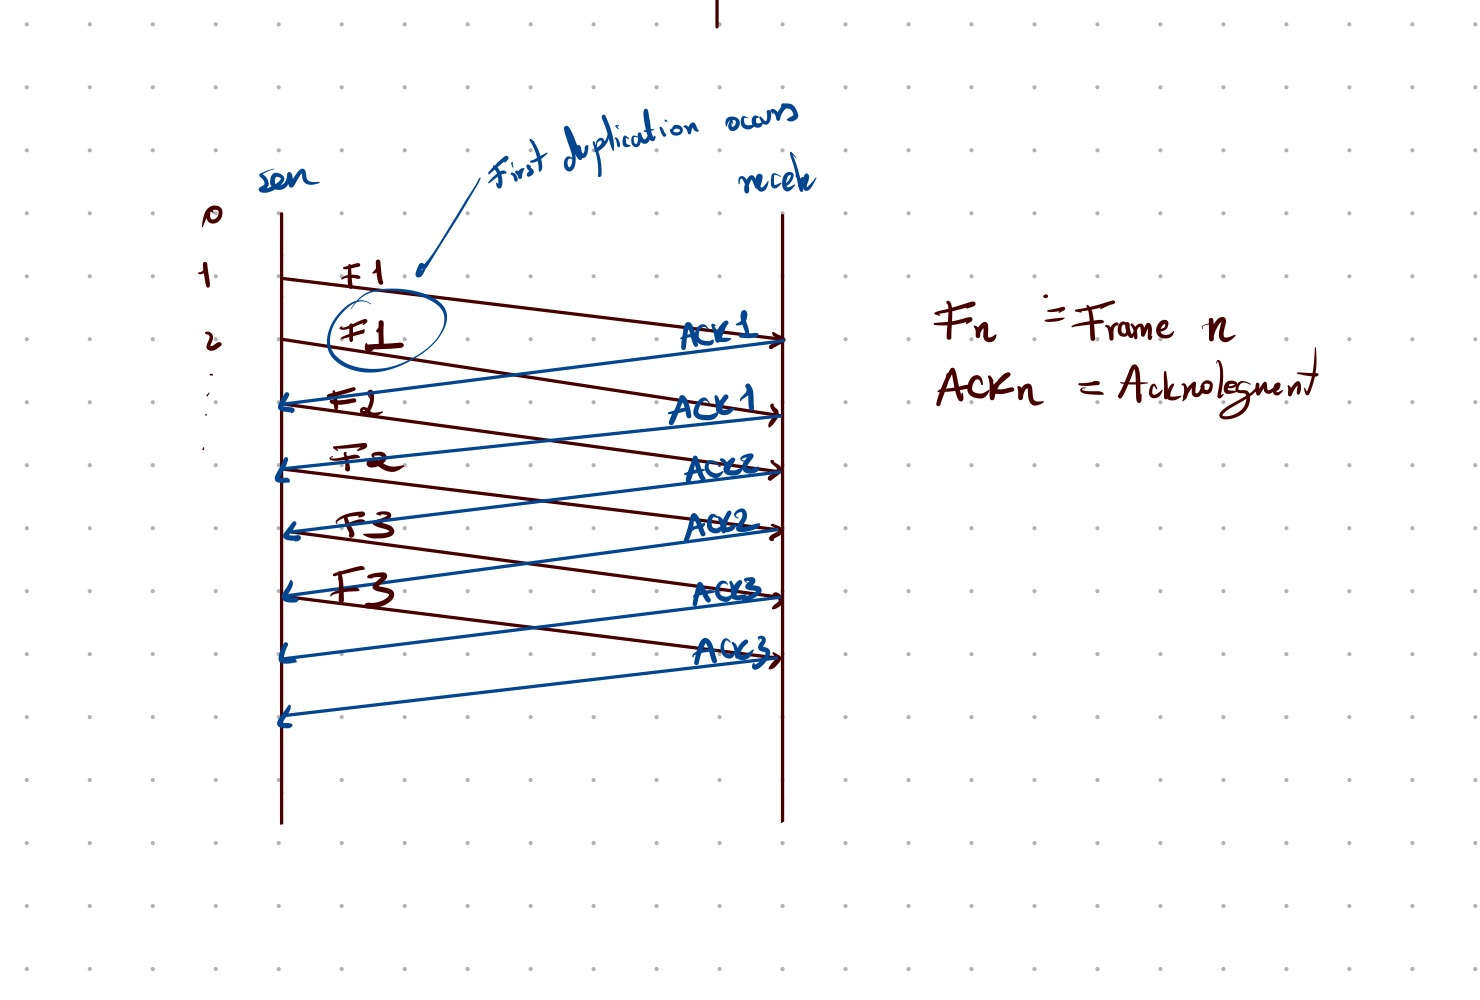
\includegraphics[scale=0.3]{1.JPG}
  \end{center}
  \caption{Timeline of the Sorcerer's Apprentice Bug}
  \label{fig:}
  \end{figure}

  The idea is that the duplications will continue till the package is done
  trasmitting, meaning that when a frame or packet is duplicated then all the
  others will be duplicated
\newpage
\item The timeline will look almost exactly but there is a reason for
  duplicating a frame
  \begin{figure}[h]
  \begin{center}
    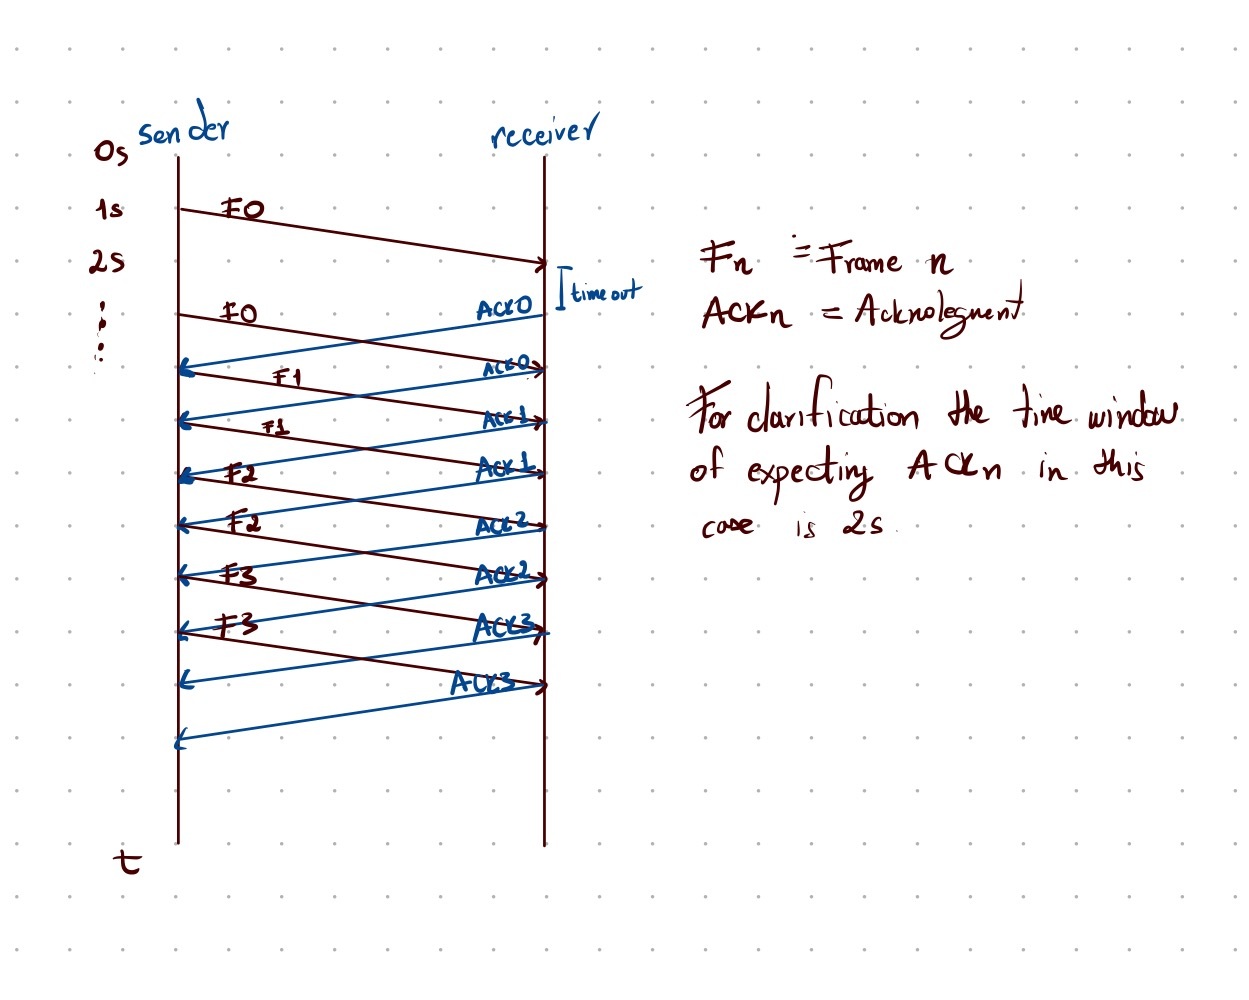
\includegraphics[scale=0.3]{2.JPG}
  \end{center}
  \caption{Timeline of the Sorcerer's Apprentice Bug}
  \label{fig:2}
  \end{figure}

  Same idea, some of the like likely causes
  \begin{itemize}
    \item Collision with other frames
    \item Maybe not enough space in the receiver to accept the package, so it
      has a timeout to manage and that can cause a little timeout
    \item External factors as loss of power, or maybe a reboot
  \end{itemize}
\end{enumerate} 
\newpage
\begin{ex}
Draw a timeline diagram for the sliding window algorithm with SWS = RWS = 4 frames for the 
following two situations. Assume the receiver sends a duplicate acknowledgement if it does not receive 
the expected frame. For example, it sends DUPACK[2] when it expects to see FRAME[2] but receives 
FRAME[3] instead. Also, the receiver sends a cumulative acknowledgment after it receives all the 
outstanding frames. For example, it sends ACK[5] when it receives the lost frame FRAME[2] after it 
already received FRAME[3], FRAME[4], and FRAME[5]. Use a timeout interval of about 2 × RTT.
\begin{enumerate}
  \item Frame 2 is lost. Retransmission takes place upon timeout (as usual).
  \item Frame 2 is lost. Retransmission takes place either upon receipt of the first DUPACK or upon 
timeout. Does this scheme reduce the transaction time? Note that some end-to-end protocols (e.g., 
\end{enumerate}
\end{ex}
\textit{ Sol. }
\begin{enumerate}
  \item Upon timeout the retransmittion will happen thus
    \begin{figure}[h]
    \begin{center}
      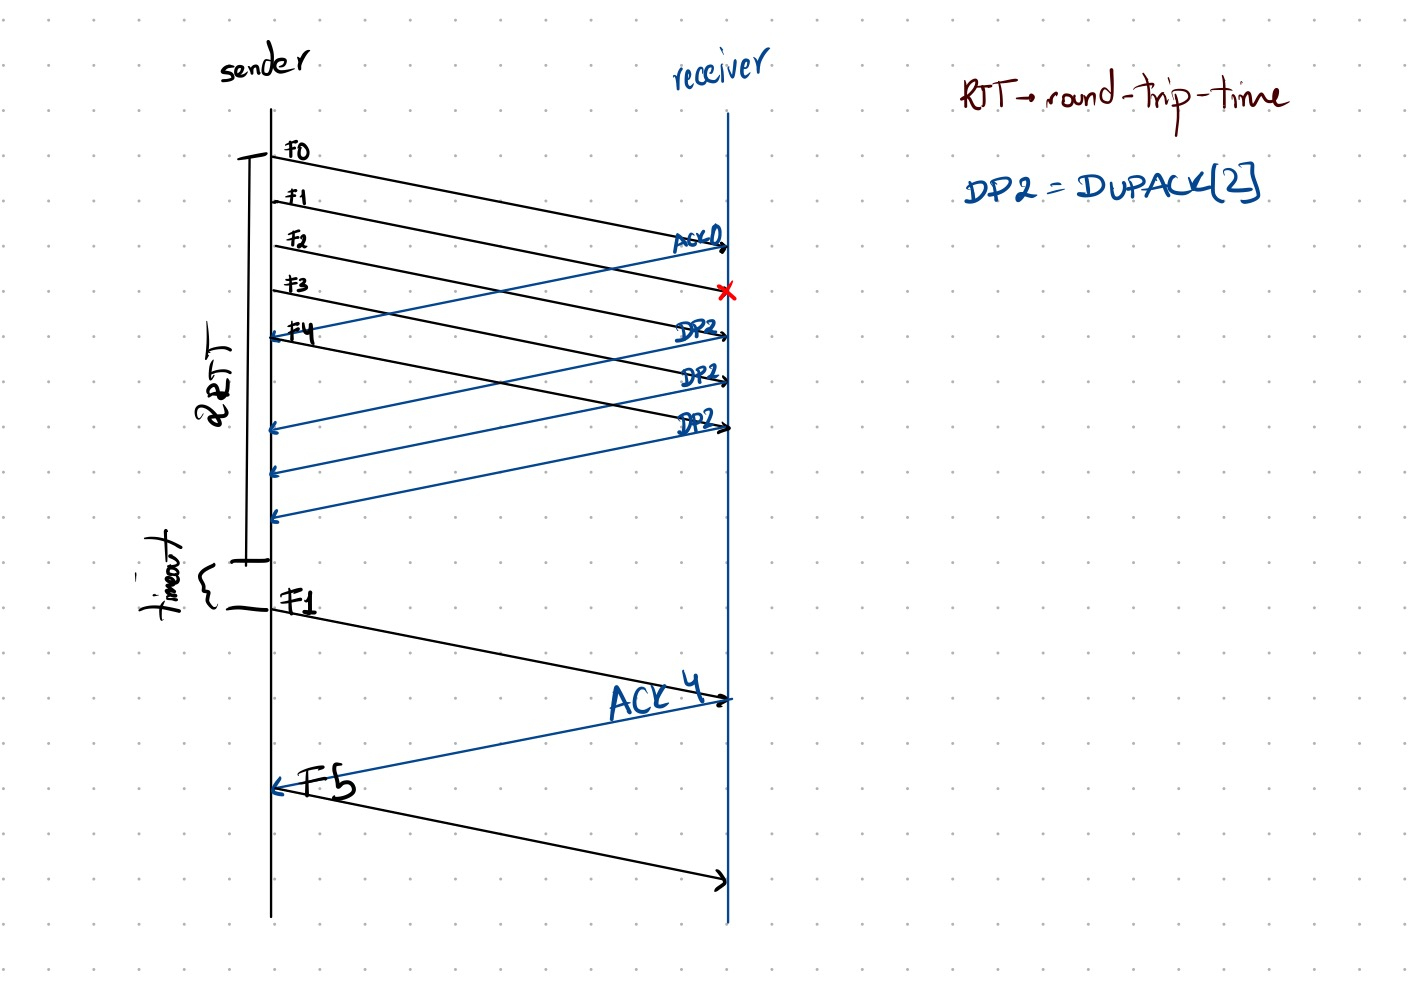
\includegraphics[scale=0.3]{5.JPG}
    \end{center}
    \label{fig:3}
    \caption{Upon timeout}
    \end{figure}
    \newpage
  \item Instantly

    \begin{figure}[h]
    \begin{center}
      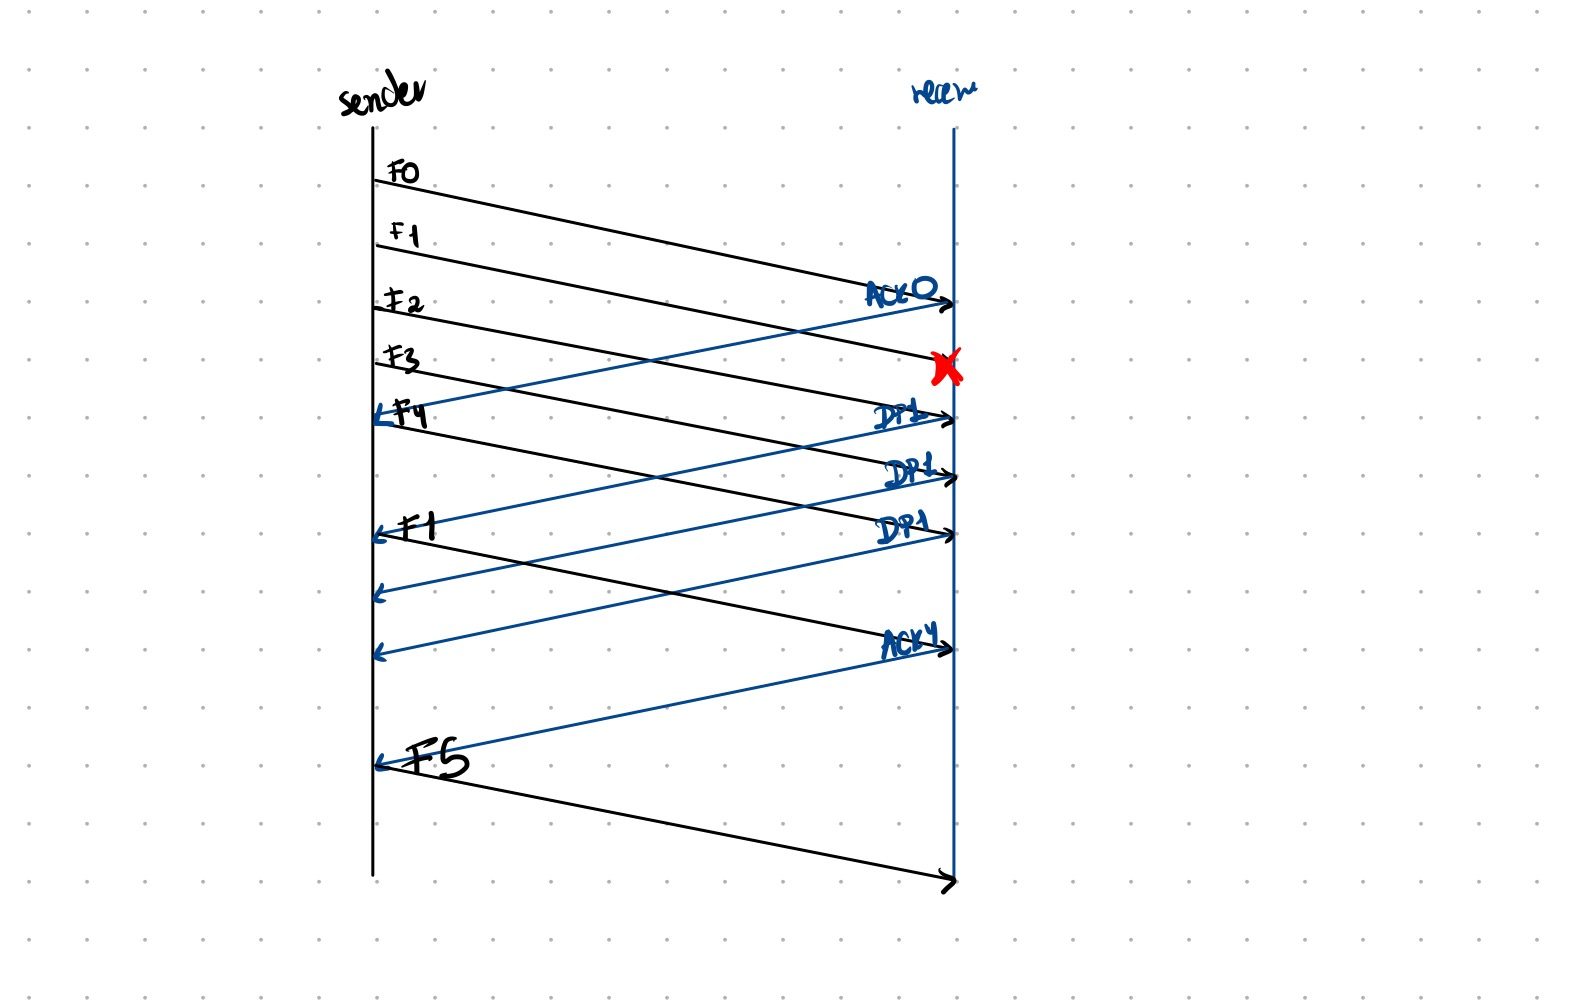
\includegraphics[scale=0.27]{3.JPG}
    \end{center}
    \caption{Instantly}
    \label{fig:4}
    \end{figure}
    Tecnically is faster
\end{enumerate}

\end{document}
